\chapter{The Theory of Regular Languages \label{chapter:regular-languages}}

\begin{figure}[h] 
\centering
  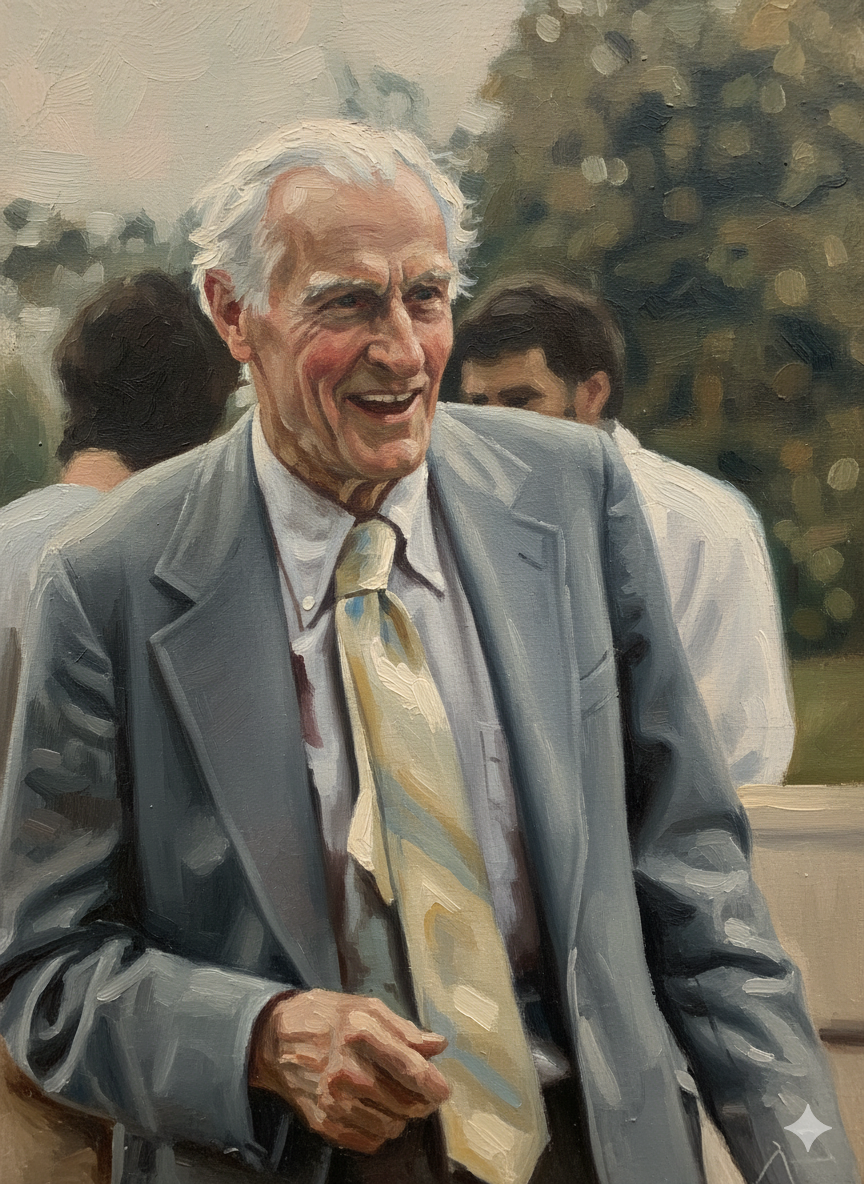
\includegraphics[width=10.5cm]{Abbildungen/Stephen_Cole_Kleene.png}
\caption{Stephen Cole Kleene, the father of regular languages.}
\label{fig:chapter-image}
\end{figure}

A formal language $L \subseteq \Sigma^*$ is called a \blue{regular language} \index{regular language}
if there is a regular expression $r$ such that the language $L$ is specified by $r$, i.e.~if
\\[0.2cm]
\hspace*{1.3cm}
$L = L(r)$ 
\\[0.2cm]
holds.  In Chapter \ref{chapter:finite-state-machines} we have shown that the regular languages
are those languages that are recognized by a finite state machine.  In this chapter, we show
that the class of regular languages has certain \blue{closure properties}:
\begin{enumerate}[(a)]
\item The \blue{union} $L_1 \cup L_2$ of two regular languages $L_1$ and $L_2$ is a regular language, too.
\item The \blue{intersection} $L_1 \cap L_2$ of two regular languages $L_1$ und $L_2$ is again a regular language.
\item The \blue{complement} \index{complement of a language} $\Sigma^* \backslash L$ of a regular language $L$
      is also a regular language.
\end{enumerate}
As an application of these closure properties we will then show how it is possible to decide whether two
regular expressions are \blue{equivalent}, i.e.~we present an algorithm that takes two regular expressions
$r_1$ and $r_2$ as input and checks, whether 
\\[0.2cm]
\hspace*{1.3cm}
$r_1 \doteq r_2$
\\[0.2cm]
holds.  After that, we discuss the \blue{limits} of regular languages.  To this end, we prove the
\href{http://en.wikipedia.org/wiki/Pumping_lemma_for_regular_languages}{\emph{pumping lemma}}.
Using the pumping lemma we will be able to show that, for example, the language
\\[0.2cm]
\hspace*{1.3cm} $\{ \mathtt{a}^n \mathtt{b}^n \mid n \in \mathbb{N} \}$
\\[0.2cm]
is not regular.  To summarize, this chapter 
\begin{itemize}
\item discusses closure properties of regular languages
\item presents an algorithm for checking the equivalence of regular expressions, and
\item shows that certain languages are not regular.
\end{itemize}


\section{Closure Properties of Regular Languages}
In this section we show that regular languages are closed under the Boolean operations
of \blue{union}, \blue{intersection} and \blue{complement}.  We start with the union.

\begin{Proposition} \label{prop:13}
  If $L_1$ and $L_2$ are regular languages, then the union of the sets $L_1$ and $L_2$, which is the set $L_1 \cup L_2$,
  is a regular language, too. 
\end{Proposition}

\proofEng
As $L_1$ and $L_2$ are regular languages, there exist regular expressions $r_1$ and $r_2$ such that
\\[0.2cm]
\hspace*{1.3cm}
$L_1 = L(r_1)$ \quad and \quad $L_2 = L(r_2)$
\\[0.2cm]
holds.  We define $r := r_1 + r_2$.  Then we have
\\[0.2cm]
\hspace*{1.3cm}
$L(r) = L(r_1 + r_2) = L(r_1) \cup L(r_2) = L_1 \cup L_2$.
\\[0.2cm]
Since $L_1 \cup L_2$ is the language that is generated by the regular expression $r_1 + r_2$, it is a regular language.
\qed  

\begin{Proposition} \label{satz:schnitt}
  If  $L_1$ and $L_2$ are regular languages, then the intersection of the sets $L_1$ and $L_2$, which is the
  set $L_1 \cap L_2$, is a regular language, too. 
\end{Proposition}

\proofEng
While the proof of Proposition \ref{prop:13} follows directly from the definition of regular expressions,
we have to do a little more work here. In the previous chapter we saw that for every regular expression
$r$ there is an equivalent deterministic finite state machine $F$, which accepts the language specified by $r$,
and we can also assume that this \textsc{Dfa} is complete. Let $r_1$ and $r_2$ be the regular expressions that
define the languages $L_1$ and $L_2$, i.e.~we have
\\[0.2cm]
\hspace*{1.3cm}
$L_1 = L(r_1)$ \quad und \quad $L_2 = L(r_2)$.
\\[0.2cm]
First, we construct two complete deterministic \textsc{Fsm}s
$F_1$ and $F_2$ that accept these languages, i.e.~such that we have
\\[0.2cm]
\hspace*{1.3cm}
$L(F_1) = L_1(r_1)$ \quad and \quad $L(F_2) = L_2(r_2)$.
\\[0.2cm]
Our goal is to construct a finite state machine $F$ such that $F$ accepts the language
$L_1 \cap L_2$ and nothing else.  As every finite state machine can be converted into an equivalent regular
expression we will then have shown that the language
$L_1 \cap L_2$ is regular.  We will use the \textsc{Fsm}s $F_1$ and $F_2$ to construct $F$.
Assume that
\\[0.2cm]
\hspace*{1.3cm}
$F_1 = \langle Q_1, \Sigma, \delta_1, q_1, A_1 \rangle$ \quad and \quad
$F_2 = \langle Q_2, \Sigma, \delta_2, q_2, A_2 \rangle$
\\[0.2cm]
holds.  We define $F$ as follows:
\\[0.2cm]
\hspace*{1.3cm}
$F := \langle Q_1 \times Q_2, \Sigma, \delta, \pair(q_1,q_2), A_1 \times A_2 \rangle$,
\\[0.2cm]
where the state transition function 
\\[0.2cm]
\hspace*{1.3cm}
 $\delta: (Q_1 \times Q_2) \times \Sigma \rightarrow Q_1 \times Q_2$ 
\\[0.2cm]
is defined as
\\[0.2cm]
\hspace*{1.3cm}
$\delta\bigl( \pair(p_1, p_2), c \bigr) := \bigl\langle\delta_1(p_1,c), \delta_2(p_2,c)\bigr\rangle$.
\\[0.2cm]
Effectively, the \textsc{Fsm} $F$ runs the \textsc{Fsm} $F_1$ and $F_2$ in parallel.  In order to do so, the
states of $F$ are pairs of the form $\pair(p_1,p_2)$ where $p_1$ is a state from $F_1$ and $p_2$ is a state from
$F_2$ and the transition function $\delta$ computes the state $\bigl\langle\delta_1(p_1,c), \delta_2(p_2,c)\bigr\rangle$
by simultaneously computing the next states of $p_1$ and $p_2$ in the \textsc{Fsm}s $F_1$ and $F_2$ when these
\textsc{Fsm}s read the character $c$.  A string $s$ is accepted by $F$ if and only if
both $F_1$ and  $F_2$ accept $s$.  Therefore, the set $A$ of accepting states of the \textsc{Fsm} $F$ is defined as:
\\[0.2cm]
\hspace*{1.3cm}
$A := \bigl\{ \pair(p_1,p_2) \in Q_1 \times Q_2 \mid p_1 \in A_1 \wedge p_2 \in A_2 \bigr\} = A_1 \times A_2$.
\\[0.2cm]
Then for all $s \in \Sigma^*$ we have:
$$
\begin{array}[t]{cl}
                & s \in L(F)                                                           \\[0.1cm]
\Leftrightarrow & \delta(\pair(q_1,q_2), s) \in A                                      \\[0.1cm]
\Leftrightarrow & \langle \delta_1(q_1,s), \delta_2(q_2, s) \rangle \in A_1 \times A_2 \\[0.1cm]
\Leftrightarrow & \delta_1(q_1,s) \in A_1 \;\wedge\;  \delta_2(q_2, s) \in A_2             \\[0.1cm]
\Leftrightarrow & s \in L(F_1) \;\wedge\;  s \in L(F_2)                                    \\[0.1cm]
\Leftrightarrow & s \in L(F_1) \cap L(F_2)                                             \\[0.1cm]
\Leftrightarrow & s \in L_1 \cap L_2                                                 
\end{array}
$$
Therefore we have shown that
\\[0.2cm]
\hspace*{1.3cm}
 $L(F) = L_1 \cap L_2$ 
\\[0.2cm]
and this completes the proof. \qed

\remarkEng
In principle it would be possible to define a function
\\[0.2cm]
\hspace*{1.3cm}
$\wedge: \textsl{RegExp} \times \textsl{RegExp} \rightarrow \textsl{RegExp}$
\\[0.2cm]
that takes two regular expressions $r_1$ and $r_2$ and returns a regular expression  $r_1 \wedge r_2$ such that
we have
\\[0.2cm]
\hspace*{1.3cm}
$L(r_1 \wedge r_2) = L(r_1) \cap L(r_2)$.
\\[0.2cm]
To compute $r_1 \wedge r_2$ we would first compute non-deterministic \textsc{Fsm}s  $F_1$ and $F_2$ such that
\\[0.2cm]
\hspace*{1.3cm}
$L(F_1) = L(r_1)$ \quad and \quad $L(F_2) = L(r_2)$
\\[0.2cm] 
holds.  Then we would transform the \textsc{Fsm}s $F_1$ and $F_2$ into equivalent deterministic 
\textsc{Fsm}s $\mathtt{det}(F_1)$ and $\mathtt{det}(F_2)$.  After that, we would build
the extended Cartesian product of $\mathtt{det}(F_1)$ and $\mathtt{det}(F_2)$ as shown above. 
Finally, we would convert the \textsc{Fsm} $\mathtt{det}(F_1) \times\mathtt{det}(F_2)$ into an equivalent
regular expression.  However, most of the time the resulting regular expression would be absurdly large. 
Therefore, it is not practical to implement the function $\wedge$.
\eox


\begin{Proposition}
  If $L$ is a regular language with the alphabet $\Sigma$, then the \blue{complement} \index{complement of a language}
  of $L$, which is defined as the language $\Sigma^* \backslash L$, is regular.
\end{Proposition}

\proofEng
We assume that $r$ is a regular expression describing the language $L$, i.e.~$L=L(r)$. 
We construct a non-deterministic \textsc{Fsm} $F$ such that $L(F) = L(r) = L$.  
We transform this non-deterministic \textsc{Fsm} into the deterministic \textsc{Fsm} $\mathtt{det}(F)$ as discussed
in the previous chapter and note that this \textsc{Dfa} is complete.
Assume that we then have
\\[0.2cm]
\hspace*{1.3cm} $\mathtt{det}(F) = \langle Q, \Sigma, \delta, q_0, A \rangle$.
\\[0.2cm]
We define the deterministic \textsc{Fsm} $\overline{\mathtt{det}(F)}$ as follows:
\\[0.2cm]
\hspace*{1.3cm} $\overline{\mathtt{det}(F)} = \langle Q, \Sigma, \delta, q_0, Q \backslash A \rangle$.
\\[0.2cm]
i.e.~the set of accepting states of $\overline{\mathtt{det}(F)}$ is the complement of the set of accepting
states of $F$.  Then we have
$$
\begin{array}[t]{cl}
                  & w \in L\Bigl(\overline{\mathtt{det}(F)}\Bigr)                      \\[0.2cm]
  \Leftrightarrow & \delta^*(q_0, w) \in Q \backslash A     \\[0.2cm]
  \Leftrightarrow & \delta^*(q_0, w) \not\in A \\[0.2cm]
  \Leftrightarrow & w \not\in L\bigl(\mathtt{det}(F)\bigr) \\[0.2cm]
  \Leftrightarrow & w \not\in L(F) \\[0.2cm]
  \Leftrightarrow & w \not\in L(r) \\[0.2cm]
  \Leftrightarrow & w \not\in L \\[0.2cm]
  \Leftrightarrow & w \in \Sigma^* \backslash L 
 \end{array}
$$
This shows that the language $\Sigma^* \backslash L$ is accepted by the \textsc{Fsm} $\overline{\mathtt{det}(F)}$
and hence it is a regular language.
 \qed

\begin{Corollary} \label{kor:mengendif}
  If $L_1$ and $L_2$ are regular languages over the common alphabet $\Sigma$, then the \blue{set difference}
  \index{set difference} $L_1 \backslash L_2$  is a regular language.
\end{Corollary}

\proofEng
A string $w$ is a member of $L_1 \backslash L_2$ iff $w$ is a member of $L_1$
and $w$ is also a member of the complement of $L_2$.  Therefore we have
\\[0.2cm]
\hspace*{1.3cm}
$L_1 \backslash L_2 = L_1 \cap (\Sigma^* \backslash L_2)$,
\\[0.2cm]
The previous proposition shows that for a regular language $L_2$ the complement
$\Sigma^* \backslash L_2$ is also a regular language.  Since the intersection of regular languages is regular,
too, we see that $L_1 \backslash L_2$ is also regular.
\qed
\vspace*{0.3cm}

In summary, we have demonstrated that regular languages are closed under the operations of Boolean algebra on sets.
\pagebreak


\exerciseEng
Let \(\Sigma\) be a given alphabet. For a string \(s = c_1 c_2 \ldots c_{n-1} c_n \in \Sigma^*\), the \textcolor{blue}{reversal} \index{reversal of a string} of \(s\) is denoted by \(s^R\) and is defined as follows:
\[
\hspace*{1.3cm}
s^R := c_n c_{n-1} \ldots c_2 c_1
\]
For instance, if \(s = \mathtt{abc}\), then \(s^R = \mathtt{cba}\). The reversal \(L^R\) of a language \(L \subseteq \Sigma^*\) is formally defined as:
\[
\hspace*{1.3cm}
L^R := \{ s^R \mid s \in L \}
\]
Subsequently, let us consider a language \(L \subseteq \Sigma^*\) that is regular. Your task is to prove that \(L^R\) is also a regular language. \eox


\section{Recognizing Empty Languages \label{section:leer}}
In this section we develop an algorithm that takes a deterministic \textsc{Fsm}
\\[0.2cm]
\hspace*{1.3cm}
$F = \langle Q, \Sigma, \delta, q_0, A \rangle$
\\[0.2cm]
as its input and then checks, whether the language accepted by $F$ is empty, i.e.~it checks whether 
$L(F) = \{\}$.  To this end we interpret the \textsc{Fsm} $F$ as a directed graph.  The nodes of this graph are the
states of the set $Q$ and for two states $q_1$ and
$q_2$ there is an edge  $q_1$ from to $q_2$ iff there exists a character $c \in \Sigma$, such that $\delta(q_1,
c) = q_2$.  
The language $L(F)$ is empty if and only if this graph has no path that starts in the state
$q_0$ and leads to an accepting state.

Therefore, in order to answer the question whether $L(F) = \{\}$ holds, we have to compute the set $R$
of all those states that are \blue{reachable} from the start state $q_0$.  The computation of the set $R$ of
all reachable states can be done iteratively as follows:
\begin{enumerate}
\item $q_0 \in R$, \quad because the start state is obviously reachable from the start state.
\item $p_1 \in R \wedge \delta(p_1,c) = p_2 \;\rightarrow\; p_2 \in R$,

      because if $p_1$ is reachable form $q_0$ and there is a transition from $p_1$ to $p_2$ while reading the
      character $c$, then $p_2$ is reachable from $q_o$.

      This last step is repeated until there are no more states that can be added to the set $R$.
\end{enumerate}
Then we have $L(F) = \{\}$ if and only if none of the accepting states is reachable, i.e.~we have
\\[0.2cm]
\hspace*{1.3cm}
$L(F) = \{\} \;\Leftrightarrow\; R \cap A = \{\}$.
\\[0.2cm]
Hence we now have an algorithm for checking whether $L(F) = \{\}$ holds:
We compute the states that are reachable from the start state $q_0$ and then we check whether this set
contains any accepting states.

\remarkEng
If the regular language  $L$ is not specified via an \textsc{Fsm} $F$, but rather is defined
via a regular expression $r$, then there is a simple recursive algorithm for checking whether 
$L(r)$ is empty:
\begin{enumerate}
\item $L(\emptyset) = \{\}$.
\item $L(\varepsilon) \not= \{\}$.
\item $L(c) \not= \{\}$ \quad for all $c \in \Sigma$.
\item $L(r_1 \cdot r_2) = \{\} \;\Leftrightarrow\; L(r_1) = \{\} \vee L(r_2) = \{\}$.
\item $L(r_1 + r_2) = \{\} \;\Leftrightarrow\; L(r_1) = \{\} \wedge L(r_2) = \{\}$.
\item $L(r^*) \not= \{\}$. \eox
\end{enumerate}


\section{Equivalence of Regular Expressions}
In Chapter \ref{chapter:regular-expressions} we had defined two regular expressions $r_1$ and $r_2$ to be \blue{equivalent} 
(written $r_1 \doteq r_2$), if the languages specified by $r_1$ and $r_2$ are identical:
\\[0.2cm]
\hspace*{1.3cm}
$r_1 \doteq r_2 \stackrel{\mbox{\scriptsize def}}{\Longleftrightarrow} L(r_1) = L(r_2)$. 
\\[0.2cm]
In this section, we present an algorithm that takes two regular expressions $r_1$ and $r_2$ as input and then
checks whether $r_1 \doteq r_2$ holds. 


\begin{Theorem}
  If $r_1$ and $r_2$ are regular expressions, then the question whether $r_1 \doteq r_2$ holds is decidable.
\end{Theorem}

\proofEng
We present an algorithm that decides whether $L(r_1) = L(r_2)$ holds.  First, we observe that the sets
$L(r_1)$ and $L(r_2)$ are identical iff the set differences $L(r_2) \backslash L(r_1)$ and $L(r_1) \backslash L(r_2)$
are both empty:
\begin{eqnarray*}
                  L(r_1) = L(r_2) 
&\Leftrightarrow& L(r_1) \subseteq L(r_2)         \;\wedge\; L(r_2) \subseteq L(r_1)          \\
&\Leftrightarrow& L(r_1) \backslash L(r_2) = \{\} \;\wedge\; L(r_2) \backslash L(r_1) = \{\}  
\end{eqnarray*}
Next, assume that $F_1$ and $F_2$ are deterministic \textsc{Fsms} such that
\\[0.2cm]
\hspace*{1.3cm}
$L(F_1) = L(r_1)$ \quad and \quad $L(F_2) = L(r_2)$
\\[0.2cm]
holds.  We have seen in Chapter \ref{chapter:finite-state-machines} how $F_1$ and $F_2$ can be
constructed from $r_1$ and $r_2$. According to the corollary \ref{kor:mengendif} the languages
$L(r_1) \backslash L(r_2)$ and $L(r_2) \backslash L(r_1)$ are regular and we have seen how to
construct \textsc{Fsm}s $F_{1,2}$ and $F_{2,1}$ such that
\\[0.2cm]
\hspace*{1.3cm}
$L(r_1) \backslash L(r_2) = L(F_{1,2})$ \quad and \quad $L(r_2) \backslash L(r_1) = L(F_{2,1})$ 
\\[0.2cm]
holds.  Hence we have
\\[0.2cm]
\hspace*{1.3cm}
$r_1 \doteq r_2 \;\Leftrightarrow\; L(F_{1,2}) = \{\} \wedge  L(F_{2,1}) = \{\}$
\\[0.2cm]
and according to Section \ref{section:leer} this question is decidable by checking whether any of
the accepting states of $F_{1,2}$ or $F_{2,1}$ are reachable from the start state.
\qed

\remarkEng
The Jupyter notebook \texttt{Equivalence.ipynb}, which is available at
\\[0.2cm]
\hspace*{0.3cm}
\href{https://github.com/karlstroetmann/Formal-Languages/blob/master/Python/Chapter-04-05/09-Equivalence.ipynb}{https://github.com/karlstroetmann/Formal-Languages/blob/master/Python/Chapter-04-05/09-Equivalence.ipynb}
\\[0.2cm]
implements this algorithm.

\section{Limits of Regular Languages}
In this section we present a theorem that can be used to show that certain languages are
\underline{not} regular.  This theorem is known as the 
\href{https://en.wikipedia.org/wiki/Pumping_lemma_for_regular_languages}{\blue{pumping lemma for regular languages}}.

\begin{Theorem}[\href{https://en.wikipedia.org/wiki/Pumping_lemma_for_regular_languages}{Pumping Lemma for
    Regular Languages}, Michael Rabin and Dana Scott 1959, \cite{rabin:1959}] \lb
  \index{pumping lemma for regular languages} \index{Pumping Lemma for regular languages}
  Assume $L$ is a regular language.  Then there exists a natural number $n \in \mathbb{N}$ such that
  every string $s \in L$ that has a length of at least $n$ can be split into three substrings $u$,
  $v$, and $w$ such that the following holds:
  \begin{enumerate}
  \item $s= uvw$,
  \item $v \not= \lambda$,
  \item $|uv| \leq n$,
  \item $\forall h \in \mathbb{N}: uv^hw \in L$.
  \end{enumerate}
  This theorem can be written as a single formula:  If $L$ is a regular language, then 
  \\[0.2cm]
  \hspace*{1.3cm}
  $\exists n \in \mathbb{N}:\forall s \in L : \bigl(|s| \geq n \rightarrow \exists u,v,w\in \Sigma^* :
   s = uvw \wedge v \not= \lambda \wedge |uv| \leq n \wedge 
    \forall h \in \mathbb{N}: uv^h w \in L
   \bigr)
  $.
\end{Theorem}

\proofEng
As $L$ is a regular language, there exists a deterministic \textsc{Fsm}
\\[0.2cm]
\hspace*{1.3cm}
$F = \langle Q, \Sigma, \delta, q_0, A \rangle$,
\\[0.2cm]
such that $L = L(F)$.  The number $n$ whose existence is claimed in the Pumping Lemma is defined as
the number of states of $F$: 
\\[0.2cm]
\hspace*{1.3cm}
$n := \textsl{card}(Q)$.
\\[0.2cm]
Next, assume a string $s \in L$ is given such that $|s| \geq n$.  Define $m := |s|$. Then there are $m$
characters $c_i$ such that
\\[0.2cm]
\hspace*{1.3cm}
$s = c_1 c_2 \cdots c_m$.
\\[0.2cm]
Since $|s| \geq n$, we have $m \geq n$.  On reading the characters $c_i$ the \textsc{Fsm} changes its
states as follows:
\\[0.2cm]
\hspace*{1.3cm}
$q_0 \stackrel{c_1}{\longmapsto} q_1 \stackrel{c_2}{\longmapsto} q_2 \stackrel{c_3}{\longmapsto} \cdots \stackrel{c_m}{\longmapsto} q_m$,
\\[0.2cm]
i.e.~on reading the character $c_{i+1}$ in the state $q_i$ the \textsc{Fsm} switches into the state $q_{i+1}$
for all $i=0,\cdots,m-1$.
Since we have  $s \in L$ we conclude that  $q_m$ must be an accepting state, i.e.~$q_m \in A$.
As $m \geq n$ and $n$ is the total number of states of $F$, not all of the states 
\\[0.2cm]
\hspace*{1.3cm}
$q_0$, $q_1$, $q_2$, $\cdots$, $q_m$
\\[0.2cm]
can be different.
Because of
\\[0.2cm]
\hspace*{1.3cm}
$\textsl{card}\bigl(\{0,1,\cdots,n\}\bigr) = n+1$
\\[0.2cm]
we know, that even in the list
\\[0.2cm]
\hspace*{1.3cm}
$[q_0,q_1,q_2,\cdots, q_{n}]$
\\[0.2cm]
at least one state has to occur at least twice.  Hence there are natural numbers $k, l \in \{0,\cdots,n\}$ such that
\\[0.2cm]
\hspace*{1.3cm}
$q_k = q_l \wedge k < l$.
\\[0.2cm]
Next, we define the strings $u$, $v$, and $w$ as follows:
\\[0.2cm]
\hspace*{1.3cm}
$u := c_1 \cdots c_k$, \quad $v := c_{k+1} \cdots c_l$, \quad and \quad $w := c_{l+1} \cdots c_{m}$.
\\[0.2cm]
As $k < l$ we have that $v \not= \lambda$ and $l \leq n$ implies $|uv| \leq n$.
Furthermore, we have the following:
\begin{enumerate}
\item Reading the string $u$ changes the state of the \textsc{Fsm} $F$ from the start state $q_0$ to
      the state $q_k$, we have
      \begin{equation}
        \label{eq:pumping1}
        q_0 \stackrel{u}{\longmapsto} q_k.    
      \end{equation}
\item Reading the string $v$ changes the state of the \textsc{Fsm} $F$ from the state $q_k$ to the
      state $q_l$.  As we have $q_l = q_k$, this implies
      \begin{equation}
        \label{eq:pumping2}
      q_k \stackrel{v}{\longmapsto} q_k.        
      \end{equation}
\item Reading the string $w$ changes the state of the \textsc{Fsm} $F$ from the state  $q_l = q_k$
      to the accepting state $q_m$:
      \begin{equation}
        \label{eq:pumping3}
        q_k \stackrel{w}{\longmapsto} q_m.        
      \end{equation}
\end{enumerate}
From $q_k \stackrel{v}{\longmapsto} q_k$ we conclude
\\[0.2cm]
\hspace*{1.3cm}
$q_k \stackrel{v}{\longmapsto} q_k \stackrel{v}{\longmapsto} q_k$, \quad hence \quad $q_k \stackrel{v^2}{\longmapsto} q_k$.
\\[0.2cm]
As we can repeat reading $v$ in state $q_k$ any number of times, we have
\begin{equation}
  \label{eq:pumping4}
  q_k \stackrel{v^h}{\longmapsto} q_k  \quad \mbox{for all $h \in \mathbb{N}$.}
\end{equation}
Combining the equations (\ref{eq:pumping1}), (\ref{eq:pumping3}), and (\ref{eq:pumping4})  we have
\\[0.2cm]
\hspace*{1.3cm}
$q_0 \stackrel{u}{\longmapsto} q_k \stackrel{v^h}{\longmapsto} q_k \stackrel{w}{\longmapsto} q_m$.
\\[0.2cm]
This can be condensed to
\\[0.2cm]
\hspace*{1.3cm}
$q_0 \stackrel{uv^hw}{\longmapsto} q_m$
\\[0.2cm]
and since the state $q_m$ is an accepting state we conclude that $uv^hw \in L$ holds for any $h \in \mathbb{N}$. \qed



\begin{Proposition}
  The alphabet  $\Sigma$ is defined as $\Sigma = \{ \quoted{a}, \quoted{b} \}$.
  Define the language $L$ as the set of all strings of the form $\mathtt{a}^k\mathtt{b}^k$ where $k$
  is some natural number:
  \\[0.2cm]
  \hspace*{1.3cm}
  $L = \bigl\{ \mathtt{a}^k\mathtt{b}^k \mid k \in \mathbb{N} \bigr\}$.
  \\[0.2cm]
  Then the language  $L$ is not regular.
\end{Proposition}

\proofEng
This is a proof by contradiction. We assume that $L$ is a regular language.  According to the
Pumping Lemma there exists a fixed natural number $n>0$ such that every $s \in L$ that satisfies  $|s|
\geq n$ can be written as
\\[0.2cm]
\hspace*{1.3cm}
$s = uvw$
\\[0.2cm]
where, furthermore, we have that
\\[0.2cm]
\hspace*{1.3cm}
$|uv| \leq n$, \quad $v \not= \lambda$, \quad and \quad $\forall h \in \mathbb{N}: uv^h w \in L$
\\[0.2cm]
holds.  Let us define the string $s$ as
\\[0.2cm]
\hspace*{1.3cm}
$s := \mathtt{a}^{n} \mathtt{b}^{n}$.
\\[0.2cm]
Obviously we have $|s| = 2 \cdot n \geq n$.  Hence there are strings $u$, $v$, and $w$
such that 
\\[0.2cm]
\hspace*{1.3cm}
$\mathtt{a}^{n}\mathtt{b}^{n} = uvw$, \quad $|uv| \leq n$, \quad $v \not= \lambda$, 
\quad and \quad $\forall h \in \mathbb{N}: uv^h w \in L$.
\\[0.2cm]
As $|uv| \leq n$, the string $uv$ is a prefix not only of $s$ but even of $\mathtt{a}^n$. Therefore,
and since $v \not= \lambda$ we know that the string $v$ must have the form
\\[0.2cm]
\hspace*{1.3cm}
$v = \mathtt{a}^k$ \quad for some $k \in \mathbb{N}$ such that $k > 0$.
\\[0.2cm]
If we take the formula $\forall h \in \mathbb{N}: uv^h w \in L$ and set  $h:=0$, we conclude that
\begin{equation}
  \label{eq:pumping5}
 uw \in L. 
\end{equation}
In order to facilitate our argument, we define the function
\\[0.2cm]
\hspace*{1.3cm}
$\textsl{count}: \Sigma^* \times \Sigma \rightarrow \mathbb{N}$.
\\[0.2cm]
Given a  string $t$ and a character $c$ the function $\textsl{count}(t,c)$ counts how often the
character $c$ occurs in the string $t$.  For the language  $L$ we have
\\[0.2cm]
\hspace*{1.3cm}
$t \in L \Rightarrow \textsl{count}(t,\texttt{'a'}) = \textsl{count}(t, \texttt{'b'})$. 
\\[0.2cm]
On one hand we have:
\[  
\begin{array}{lcl}
\textsl{count}(uw,\texttt{'a'}) & = & \textsl{count}(uvw,\texttt{'a'}) - \textsl{count}(v,\texttt{'a'}) \\
 & = & \textsl{count}(s,\texttt{'a'}) - \textsl{count}(v,\texttt{'a'}) \\
 & = & \textsl{count}(\mathtt{a}^n\mathtt{b}^n,\texttt{'a'}) - \textsl{count}(\mathtt{a}^k,\texttt{'a'}) \\
 & = & n - k  \\
 & < & n   \\
\end{array}
\]
But on the other hand we have
\[  
\begin{array}{lcl}
\textsl{count}(uw,\texttt{'b'}) & = & \textsl{count}(uvw,\texttt{'b'}) - \textsl{count}(v,\texttt{'b'}) \\
                               & = & \textsl{count}(s,\texttt{'b'}) - \textsl{count}(v,\texttt{'b'}) \\
 & = & \textsl{count}(\mathtt{a}^n\mathtt{b}^n,\texttt{'b'}) - \textsl{count}(\mathtt{a}^k,\texttt{'b'}) \\
                               & = & n  - 0\\
                               & = & n  
\end{array}
\]
Therefore, we have
\\[0.2cm]
\hspace*{1.3cm}
$\textsl{count}(uw,\texttt{'a'}) < \textsl{count}(uw,\texttt{'b'})$
\\[0.2cm]
and this shows that the string $uw$ is not a member of the language $L$ because for all strings in $L$ 
the number of occurrences of the character ``\texttt{a}'' is the same as the number of
occurrences of the character ``\texttt{b}''.  This contradiction shows that the language $L$ cannot
be regular.
\qed

\exerciseEng
Let us define the language $L$ as the set of all those strings that contain an equal number of 
occurrences of the characters ``\texttt{a}'' and  ``\texttt{b}'':
\\[0.2cm]
\hspace*{1.3cm}
$\ds L := \bigl\{ w \in \{\texttt{'a'}, \texttt{'b'}\}^* \bigm| \texttt{count}(w, \texttt{'a'})=\texttt{count}(w, \texttt{'b'}) \bigr\}$
\\[0.2cm]
Prove that the language $L$ is not regular. \eox

\remarkEng
As the language $L$ defined in the previous exercise is not regular we can conclude that regular expressions
are unable to check even such simple questions as to whether the parentheses in an expression are balanced.
Therefore, the concept of regular expressions is not strong enough to describe the syntax of a programming language.
The next chapter introduces the notion of \blue{context-free languages}.  These languages
are powerful enough to describe modern programming languages. 

\exerciseEng
The language  $L_{\mathrm{square}}$ is the set of all strings of the form $\mathtt{a}^n$ where $n$
is a square, we have
\\[0.2cm]
\hspace*{1.3cm}
$L_{\mathrm{square}} = \bigl\{ \mathtt{a}^{m} \bigm| \exists k \in \mathbb{N}: m = k^2 \bigr\}$
\\[0.2cm]
Prove that the language  $L_{\mathrm{square}}$ is not a regular language.
\eox
\vspace*{0.1cm}

\solutionEng
The proof employs the method of contradiction. We begin by assuming that $L_{\mathrm{square}}$ is a regular
language. According to the Pumping Lemma, there exists a natural number $n > 0$ such that for any string
$s \in L_{\mathrm{square}}$ with $|s| \geq n$, the string can be decomposed into three parts $u$, $v$, and $w$ 
satisfying the following conditions:  
\begin{enumerate}
\item $s = uvw$,
\item $|uv| \leq n$,
\item $v \not= \lambda$,
\item $\forall h \in \mathbb{N}: uv^hw \in L_{\mathrm{square}}$. 
\end{enumerate} 
Let us define $s := a^{n^2}$.  We have $s \in L_{\mathrm{square}}$ and we see that
\[ |s| = \big| a^{n^2} \big| = n^2 \geq n. \]
Hence there have to be strings $u$, $v$ and $w$ such that $s = uvw$ and $u$, $v$, and $w$ have
the properties specified above.
As '$\mathtt{a}$' is the only character that occurs in $s$, the strings $u$, $v$, and $w$ also contain only this character.
Hence there must be natural numbers $x$, $y$, and $z$ such that 
\[ u = a^x,\; v = a^y\; \mbox{und}\; w = a^z \]
holds.  Then we have the following.
\begin{enumerate}[(a)]
\item The partition  $s = uvw$ has the form $a^{n^2} = a^xa^ya^z$ and hence we have
      \begin{equation}
        \label{eq:e1}
         n^2 = x + y + z.     
      \end{equation}
\item The inequality $|uv| \leq n$ implies $x +y \leq n$, which implies
      \begin{equation}
        \label{eq:e2}
        y \leq n.
      \end{equation}
\item From the condition $v \not= \lambda$ we get
      \begin{equation}
        \label{eq:e3}
        y > 0.
      \end{equation}
\item The formula $\forall h \in \mathbb{N}: uv^hw \in L_{\mathrm{square}}$ implies
      \begin{equation}
        \label{eq:e4}
        \forall h \in \mathbb{N}: a^xa^{y\cdot h}a^z \in L_{\mathrm{square}}. 
      \end{equation}
\end{enumerate}
In particular, this must hold for $h=2$:
\[ a^xa^{y\cdot 2}a^z \in L_{\mathrm{square}}.  \]
According to the definition of $L_{\mathrm{square}}$ there is a natural number $k$ such that
\begin{equation}
  \label{eq:e5}
  x + 2\cdot y + z = k^2.
\end{equation}
If we add $y$ on both sides of equation (\ref{eq:e1}) we get
\[ n^2 + y = x + 2\cdot y + z = k^2. \]
Because of $y > 0$ this implies
\begin{equation}
  \label{eq:e6}
  n < k.    
\end{equation}
On the other hand we have
\[ 
\begin{array}[t]{lcll}
 k^2  & =    & x + 2 \cdot y + z       & \mbox{according to (\ref{eq:e5}})   \\
      & =    & x + y + z + y           &                                       \\
      & \leq & x + y + z + n           & \mbox{according to (\ref{eq:e2}}) \\
      & =    & n^2 + n                 & \mbox{according to (\ref{eq:e1}})   \\
      & <    & n^2 + 2 \cdot n + 1     & \mbox{since $n+1 > 0$}                   \\ 
      & =    & (n + 1)^2               
\end{array}
\]
This shows that  $k^2 < (n+1)^2$ holds and therefore we have
\begin{equation}
  \label{eq:e7}
  k < n+1.
\end{equation}
The inequalities (\ref{eq:e6}) and (\ref{eq:e7}) imply
\[ n < k < n + 1. \]
Since $k$ is a natural number and $n$ is also a natural number this is a contradiction because there is no
natural number between  $n$ and $n+1$.
\qed

% \renewcommand{\labelenumi}{(\alph{enumi})}
% \exerciseEngStar
% The language $L$ is defined as
% \\[0.2cm]
% \hspace*{1.3cm}
% $L := \{ \mathtt{a}^m \mathtt{b}^n \mathtt{c}^n \mid m,n \in \mathbb{N} \} \cup 
%       \{ \mathtt{b}^m \mathtt{c}^n \mid m,n \in \mathbb{N} \} 
% $.
% \begin{enumerate}
% \item Prove that $L$ is not regular.
% \item Prove that $L$ satisfies the pumping lemma.  \eox
% \end{enumerate}
% \renewcommand{\labelenumi}{\arabic{enumi}.}

\exerciseEng
Define $\Sigma := \{\mathtt{a}\}$.  
Prove that the language
\\[0.2cm]
\hspace*{1.3cm}
$L := \bigl\{ \mathtt{a}^p \mid \mbox{$p$ is a prime number} \bigr\}$
\\[0.2cm]
is not regular.  \eox
\vspace{0.3cm}

\noindent
\textbf{Proof}:
The proof is done by contradiction.  Assume that $L$ is regular.  According to the Pumping Lemma there is a
positive natural number $n$ such that all strings $s \in L$ that have a length of at least $n$ can be written as
\\[0.2cm]
\hspace*{1.3cm}
$s = uvw$
\\[0.2cm]
where, furthermore, the substrings $u$, $v$, and $w$ have the following properties:
\begin{enumerate}
\item $v \not= \lambda$, 
\item $|uv| \leq n$, \quad and
\item $\forall h \in \mathbb{N}: u v^h w \in L$.
\end{enumerate}
Let us choose a prime number $p$ such that $p \geq n + 2$.
Since there are infinitely many prime numbers, this
is always possible.  Next,  define $s := \mathtt{a}^p$.
Then we have $|s| = p \geq n$ and we can use the Pumping Lemma to conclude that there must be substrings $u$,
$v$, and $w$ such that
\\[0.2cm]
\hspace*{1.3cm}
$\mathtt{a}^p = uvw$ 
\\[0.2cm]
holds.
Hence the substrings $u$, $v$, and $w$ can only contain the letter ``\texttt{a}''.  Therefore there exist
natural numbers $x$, $y$, and $z$ such that
\\[0.2cm]
\hspace*{1.3cm}
$u = \mathtt{a}^x$, \quad $v = \mathtt{a}^y$, \quad and \quad $w = \mathtt{a}^z$.
\\[0.2cm]
We can conclude that  $x$, $y$, and $z$ have the following properties:
\begin{enumerate}
\item $x + y + z = p$,
\item $y \not= 0$,
\item $x + y \leq n$,
\item $\forall h \in \mathbb{N}: x + h \cdot y + z \in \mathbb{P}$.

      Here, $\mathbb{P}$ denotes the set of prime numbers.
\end{enumerate}
If we choose to define $h := x + z$ in the last formula, we get
\\[0.2cm]
\hspace*{1.3cm}
$x + (x + z)\cdot y + z \in \mathbb{P}$.
\\[0.2cm]
Because of $x + (x + z)\cdot y + z = (x + z) \cdot (1 + y)$ this leads to
\\[0.2cm]
\hspace*{1.3cm}
$(x + z) \cdot (1 + y) \in \mathbb{P}$.
\\[0.2cm]
This is impossible. As $y > 0$ the factor $1 + y$ is different from $1$
and because of $x + y \leq n$, $x + y + z = p$, and $p \geq n + 2$ it follows that
$z \geq 2$.  Hence the factor $x + z$ is also greater than $1$.  But then the product
$(x + z) \cdot (1 + y)$ is not a prime number and this contradiction shows that $L$ can not be regular.
\qed


\exerciseEng
The language $L_{\mathrm{power}}$ is the set of all strings of the form $\mathtt{a}^n$ where $n$ is a power of
$2$, i.e.~we have
\\[0.2cm]
\hspace*{1.3cm}
$L_{\mathrm{power}} = \bigl\{ \mathtt{a}^{2^k} \mid k \in \mathbb{N} \bigr\}$
\\[0.2cm]
Prove that the language $L_{\mathrm{power}}$ is not regular.
\eox

\section{Check your Understanding}
\begin{enumerate}[(a)]
\item What are the closure properties of regular languages?
\item How can we check whether two regular expressions are equivalent?
\item Give the exact wording of the \blue{Pumping Lemma}.
\item Can you prove that the language
      \\[0.2cm]
      \hspace*{1.3cm}
      $\ds L := \bigl\{ w \in \{\texttt{'a'}, \texttt{'b'}\}^* \bigm| \texttt{count}(w, \texttt{'a'})=\texttt{count}(w, \texttt{'b'}) \bigr\}$
      \\[0.2cm]
      is not regular?
\end{enumerate}

%%% Local Variables: 
%%% mode: latex
%%% TeX-master: "formal-languages.tex"
%%% End: 
